%; whizzy document
% latex beamer presentation.

%     Copyright (C) 2007 Junichi Uekawa

%     This program is free software; you can redistribute it and/or modify
%     it under the terms of the GNU General Public License as published by
%     the Free Software Foundation; either version 2 of the License, or
%     (at your option) any later version.

%     This program is distributed in the hope that it will be useful,
%     but WITHOUT ANY WARRANTY; without even the implied warranty of
%     MERCHANTABILITY or FITNESS FOR A PARTICULAR PURPOSE.  See the
%     GNU General Public License for more details.

%     You should have received a copy of the GNU General Public License
%     along with this program; if not, write to the Free Software
%     Foundation, Inc., 51 Franklin St, Fifth Floor, Boston, MA  02110-1301 USA

\documentclass[dvipdfm,17pt,times]{beamer}

%  preview (shell-command (concat "xpdf " (replace-regexp-in-string "tex$" "pdf"(buffer-file-name)) "&"))
%  presentation (shell-command (concat "xpdf -fullscreen " (replace-regexp-in-string "tex$" "pdf"(buffer-file-name)) "&"))
%  presentation-evince (shell-command (concat "evince " (replace-regexp-in-string "tex$" "pdf"(buffer-file-name)) "&"))
%  presentation-real (shell-command (concat "DISPLAY=:0.1 evince " (replace-regexp-in-string "tex$" "pdf"(buffer-file-name)) "&"))

\newcommand{\emtext}[1]{
\begin{frame}{}
 
{\Huge #1
}
\end{frame}
}


\title{what's happening with pbuilder?}
\subtitle{Debian Conference 2007}
\author{dancer@debian.org}
\date{June 2007}
\logo{\includegraphics[width=8cm]{openlogo-light.eps}}

\begin{document}
\frame{\titlepage{}}

\begin{frame}{Who is this guy?}
\begin{itemize}
 \item Junichi Uekawa, dancer@debian.org
 \item Lives in Japan, Leading Debian JP for 2007
 \item Debian Developer since 2000
 \item Interests: Audio-processing related tools, and 
       Debian quality maintenance related tools,
       Japanese localization, shared library packaging, 
       and more recently, Debian/MacBook related.
\end{itemize}
\end{frame}

\begin{frame}{Agenda?}
\begin{itemize}
 \item pbuilder
 \item pbuilder-uml
 \item cowbuilder
 \item qemubuilder
\end{itemize}
\end{frame}

\emtext{pbuilder, what is the concept?}

\emtext{What is a chroot?}

\begin{frame}{concept of a chroot}
 \includegraphics[width=0.8\hsize]{chroot.eps}\\
\texttt{\# chroot /var/cache/pbuilder/build/XXX bin/bash}
\end{frame}

\begin{frame}{concept of pbuilder}
 \includegraphics[width=1\hsize]{chroot-pbuilder.eps}\\
\texttt{\# pbuilder --XXXX}
\end{frame}

\emtext{How do I use pbuilder?}

\begin{frame}[containsverbatim]{installing pbuilder}
\begin{verbatim}
# apt-get install pbuilder
# vi /etc/pbuilderrc
# evince 
  /usr/share/doc/pbuilder/
     pbuilder-doc.pdf	
\end{verbatim}
\end{frame}

\begin{frame}{pbuilder basics}
\begin{minipage}{0.4\hsize}
\includegraphics[height=0.7\vsize]{pbuildercycle.eps}
\end{minipage}
\begin{minipage}{0.55\hsize}
\begin{itemize}
 \item done once to create base filesystem.
 \item twice a day to follow unstable updates, to revise base
       filesystem.
 \item for each package build to build Debian package inside chroot.
\end{itemize}
\end{minipage}
\end{frame}

\begin{frame}[containsverbatim]{pbuilder --create}
\begin{verbatim}
# pbuilder --create
Distribution is sid.
Building the build environment
 -> running debootstrap
/usr/sbin/debootstrap
I: Retrieving Release
I: Retrieving Packages
I: Validating Packages
	.
	.
\end{verbatim}
\end{frame}

\begin{frame}[containsverbatim]{pbuilder --update}
\begin{verbatim}
# pbuilder --update
W: /home/dancer/.pbuilderrc does not exist
Building the build Environment
 -> extracting base tarball [/var/cache/pbuilder/base.tgz]
	.
	.
\end{verbatim}
\end{frame}

\begin{frame}[containsverbatim]{pbuilder --build}
\begin{verbatim}
# pbuilder --build dsh_*.dsc
I: using fakeroot in build.
Current time: Sat Jan 20 12:03:34 JST 2007
pbuilder-time-stamp: 1169262214
Building the build Environment
 -> extracting base tarball [/home/dancer/DEBIAN/pbuilder/pbuilder/testsuite/tmp.FeeAX18779/testimage]
 -> creating local configuration
	.
	.
\end{verbatim}
\end{frame}


\begin{frame}[containsverbatim]{pbuilder --login}
\begin{verbatim}
# pbuilder --login --bindmount ${HOME}
I: using fakeroot in build.
Current time: Sat Jan 20 12:03:34 JST 2007
pbuilder-time-stamp: 1169262214
Building the build Environment
 -> extracting base tarball [/home/dancer/DEBIAN/pbuilder/pbuilder/testsuite/tmp.FeeAX18779/testimage]
 -> creating local configuration
	.
	.
\end{verbatim}
\end{frame}

\emtext{pdebuild}

\begin{frame}[containsverbatim]{pdebuild}
\begin{verbatim}
$ ls debian/rules
debian/rules
$ pdebuild
W: /home/dancer/.pbuilderrc does not exist
dpkg-buildpackage: source package is cowdancer
dpkg-buildpackage: source version is 0.26
dpkg-buildpackage: source changed by Junichi Uekawa <dancer@debian.org>
dpkg-buildpackage: source version without epoch 0.26
 fakeroot debian/rules clean
dh_testdir
dh_testroot
rm -f build-stamp configure-stamp
/usr/bin/make clean
make[1]: Entering directory `/home/dancer/DEBIAN/cowdancer/cowdancer'
rm -f *~ *.o *.lo libcowdancer.so cow-shell cowbuilder
make[1]: Leaving directory `/home/dancer/DEBIAN/cowdancer/cowdancer'
dh_clean
 dpkg-source -b cowdancer
dpkg-source: warning: source directory `./cowdancer' is not <sourcepackage>-<upstreamversion> `cowdancer-0.26'
dpkg-source: building cowdancer in cowdancer_0.26.tar.gz
	.
	.
	.
\end{verbatim}
\end{frame}

\begin{frame}{}
  \begin{minipage}{0.4\hsize}
   How do you maintain your package today?
  \end{minipage}
 \begin{minipage}{0.5\hsize}
  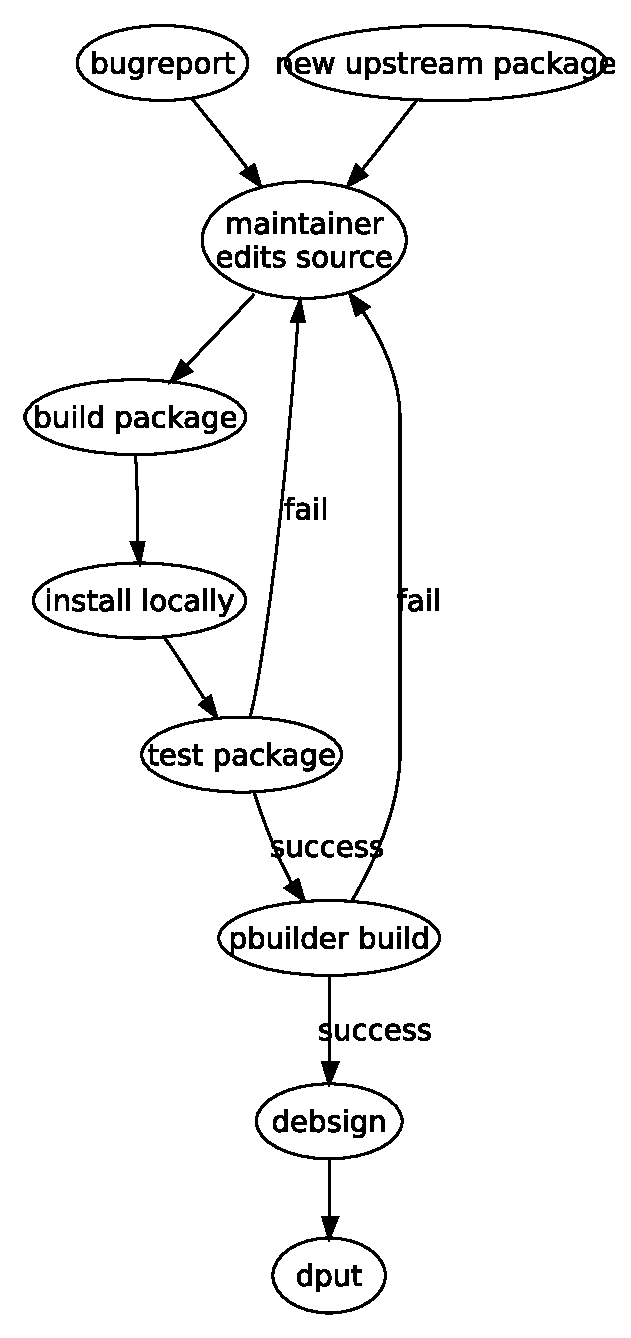
\includegraphics[height=0.95\vsize]{develcycle.eps}
 \end{minipage}
\end{frame}
 
\begin{frame}{pbuilder backend variations}
 \definecolor{titleback}{gray}{0.9}

\begin{minipage}{0.35\hsize}
  \begin{itemize}
  \item LVM
  \item UML
  \item cowdancer
  \item qemu
 \end{itemize}
\end{minipage}
\begin{minipage}{0.6\hsize}
 \colorbox{titleback}{
\begin{minipage}{1\hsize}
 Motivation
\begin{itemize}
 \item limitation in chroot segregation (process space, filesystem)
 \item COW filesystem optimization (tarball extraction slow.)
\end{itemize}
\end{minipage}
}
\end{minipage}
\end{frame}

\begin{frame}{uml}
 
 different method of segregation
 
 COW block device support

\end{frame}

\begin{frame}[containsverbatim]{cowbuilder}
 
 Speed up through use of copy-on-write filesystem.

 Just a matter of:

\begin{verbatim}
# cp -al
    /var/cache/pbuilder/base.cow 
    /var/cache/pbuilder/build/XXX
# chroot 
   /var/cache/pbuilder/build/XXX
   cow-shell 
\end{verbatim}
\end{frame}

\begin{frame}{Concepts of cowdancer}
 \begin{itemize}
  \item Usage: hardlink files, 
	\texttt{LD\_PRELOAD} libcowdancer.so;
	trap libc calls likely to cause file writes
	(open, etc) and break the hardlink.
  \item light-weight compared to other solutions (no extra partition, no
	LVM, no extra kernel modules/patches )
  \item cow-shell into it.
 \end{itemize}
\end{frame}

\begin{frame}{qemubuilder}

 Try running other architectures at your fingertips?
\end{frame}

\begin{frame}[containsverbatim]{qemubuilder example config}

\begin{verbatim}
KERNEL_IMAGE=2.6.18-4-mips-di-vmlinux
INITRD=2.6.18-4-mips-di-initrd.gz
ARCH=mips
BASEPATH=
  /var/cache/pbuilder/base-mips.qemu
\end{verbatim}
\end{frame}

\begin{frame}{qemubuilder details... create}

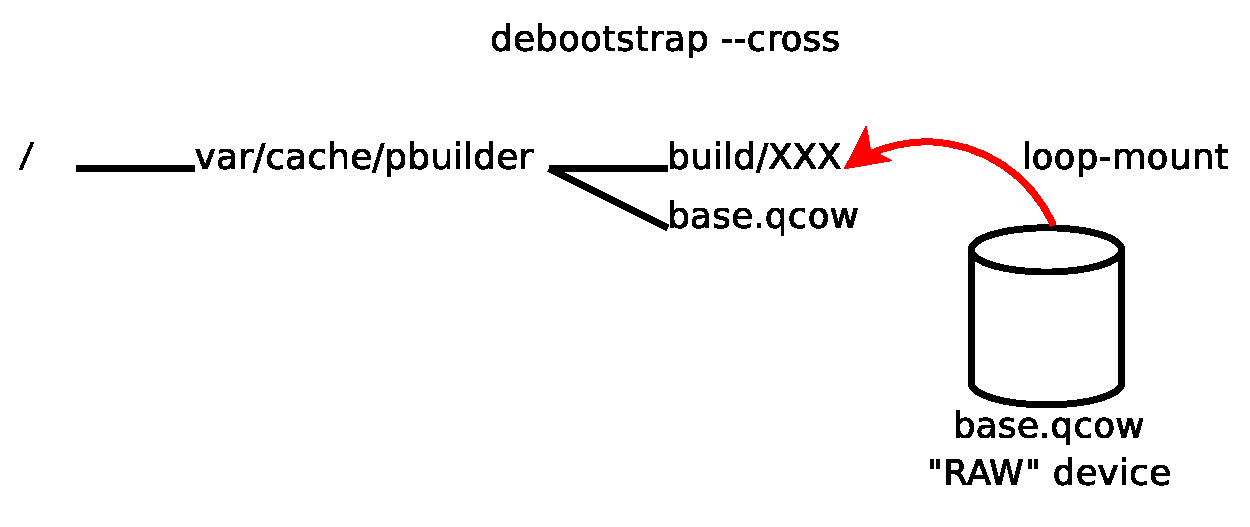
\includegraphics[width=1\hsize]{qemubuilder-create.eps}
\end{frame}

\begin{frame}{qemubuilder details... build}

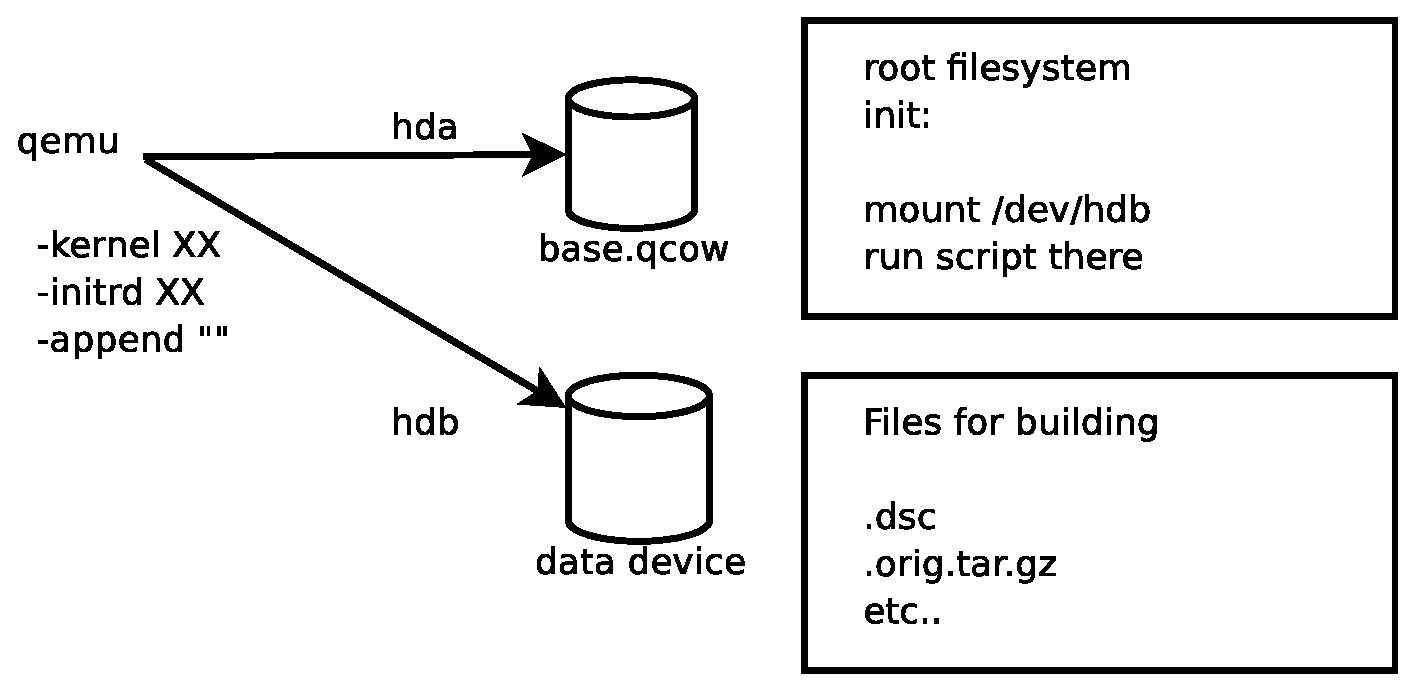
\includegraphics[width=1\hsize]{qemubuilder-build.eps}
\end{frame}

\emtext{qemubuilder --create --config mips.config}
\emtext{qemubuilder --update --config mips.config}
\emtext{qemubuilder --build --config mips.config XXX.dsc}
\begin{frame}[containsverbatim]{qemubuilder --login}
\begin{verbatim}
$ sudo qemubuilder --login --config pbuilder-qemu-mips.config
bash: /root/.pbuilderrc: No such file or directory
fsck 1.40-WIP (14-Nov-2006)
e2fsck 1.40-WIP (14-Nov-2006)
/home/dancer/tmp/base-mips.qemu: clean, 11585/393984 files, 88319/786432 blocks
1+0 records in
1+0 records out
1048576 bytes (1.0 MB) copied, 0.0229856 seconds, 45.6 MB/s
mke2fs 1.40-WIP (14-Nov-2006)
	.
	.
	.
\end{verbatim}\end{frame}

\begin{frame}[containsverbatim]{qemubuilder --login}
\begin{verbatim}
	.
	.
	.
hostname: the specified hostname is invalid
bound to 10.0.2.15 -- renewal in 35272 seconds.
bash: no job control in this shell
root@pbuilder-coreduo:/#
\end{verbatim}
\end{frame}



\begin{frame}{further ideas}
 \begin{itemize}
  \item install testing
  \item package testing
 \end{itemize}
\end{frame}

\begin{frame}{related tools}
 \begin{itemize}
  \item schroot
  \item piuparts
  \item autopkgtest
 \end{itemize}
\end{frame}

\begin{frame}{thanks to}
 \begin{itemize}
  \item Lo\"ic Minier
  \item Mattia Dongili
  \item Matt Kraai
  \item ... others as in AUTHORS / THANKS file.
 \end{itemize}
\end{frame}

\begin{frame}[containsverbatim]{References}
\begin{itemize}
 \item Information:\\
       \url{/usr/share/doc/pbuilder/pbuilder-doc.pdf}, 
       \url{http://pbuilder.alioth.debian.org/}

 \item alioth project:\\
{\scriptsize
\url{http://alioth.debian.org/projects/pbuilder}}

 \item git repository:\\
{\scriptsize
\texttt{git-clone git://git.debian.org/git/pbuilder/pbuilder.git}
}
\end{itemize}
\end{frame}


\emtext{Questions?}

\end{document}
